% !TeX encoding = UTF-8
% !TeX spellcheck = sk_SK
% !TeX root=tukedip.tex

\section{Definícia problému prenasledovania koristi a metódy jeho realizácie}
V tejto časti definujeme problém, hovoríme o spôsoboch jeho realizácie a implementujeme jednu z možných variácií pri riešení problému prenasledovania koristi pomocou multi-robotického systému.

\subsection{Analýza problému}
V tejto bakalárskej práci sa zaoberá problém prenasledovania pomocou správania viacerých robotov. Cieľom je implementovať riadiace stratégie, ktoré robotom umožňujú dosiahnuť a uzavrieť nepredvídateľne sa pohybujúcu korisť. Existuje množstvo metód
na riešenie problému kooperatívneho prenasledovania založeného na viacerých robotoch. Takéto konvenčné metódy sa delia do
dvoch kategórií, ako sú metódy založené na polohe a metódy založené senzoroch.

\vspace{3mm}

\justifying
\noindent
Lokalizovaným spôsobom je cieľové miesto známe vopred, v ktorom sa na prenasledovania cieľov používajú techniky spolupráce založené
na umelej inteligencii. Zatiaľ čo v metódach
založených na senzoroch väčšina výskumníkov používa tradičnú teóriu riadenia na vykonávanie úlohy zamerania na cieľ v
neznámom prostredí pomocou prichádzajúcich informácií zo senzora. Rozhodol som sa použiť druhú metódu založenú na
údajoch senzorov, pretože techniky založené na polohe závisia iba od informácií o polohe cieľov, čo v prostredí v
reálnom čase, kde sa polohy často menia, prakticky nie je možné.

\vspace{3mm}

\justifying
\noindent
Korisť môže vykonávať tri druhy pohybu:
\begin{enumerate}
\item Neakceleračný pohyb: korisť sa pohybuje s konštantným orientačným uhlom a rýchlosťou.
\item Zrýchľujúci pohyb: orientačný uhol koristi sa časovo mení.
\item Inteligentný pohyb: orientačný uhol koristi sa časovo mení, ale inteligentne, aby sa dalo uniknúť pred predátormi.
\end{enumerate}
Inteligentné koristi si vyžadujú prepracovanejšie stratégie. Máme nasledujúce predpoklady
\begin{enumerate}
\item Každý robot má senzorický systém, ktorý umožňuje zisťovať prekážky a odhadnúť polohu koristi podľa robota.
\item Rýchlosti robotov vyhovujú 
$v_i > v_p$, pre $i = 1, ..., N$. Kde $v_i$ - rýchlosť lovca a $v_p$ - rýchlosť koristi.
\item Roboti a korisť sa pohybujú konštantnou rýchlosťou.
\item Cesta, ktorú korisť prešla, je spojitá.
\end{enumerate}

\noindent
Realizáciu projektu možno rozdeliť na dve prakticky nezávislé časti:
\begin{itemize}
\item Režim riadenia koristi - pohyb koristi ovládaný človekom pomocou manipulátora.
\item Režim navigácie - organizácia pohybu, sledovania a prenasledovania koristi v neznámom prostredí skupinou robotov,
ktorí navzájom
komunikujú.
\end{itemize}

\subsection{Riadenie koristi}
Architektúra systému sa skladá z troch hlavných blokov:
príkazový blok, riadiaci blok a blok mobility. Príkazový blok sa skladá z klávesnice, blok mobility pozostáva z motorov,
vodičov motorov a kolies. Pri všetkých metódach ovládania používa programovací jazyk Python na odosielanie príkazov z
mikrokontroléra do ovládača motora.

\begin{figure}[ht!]
\centering
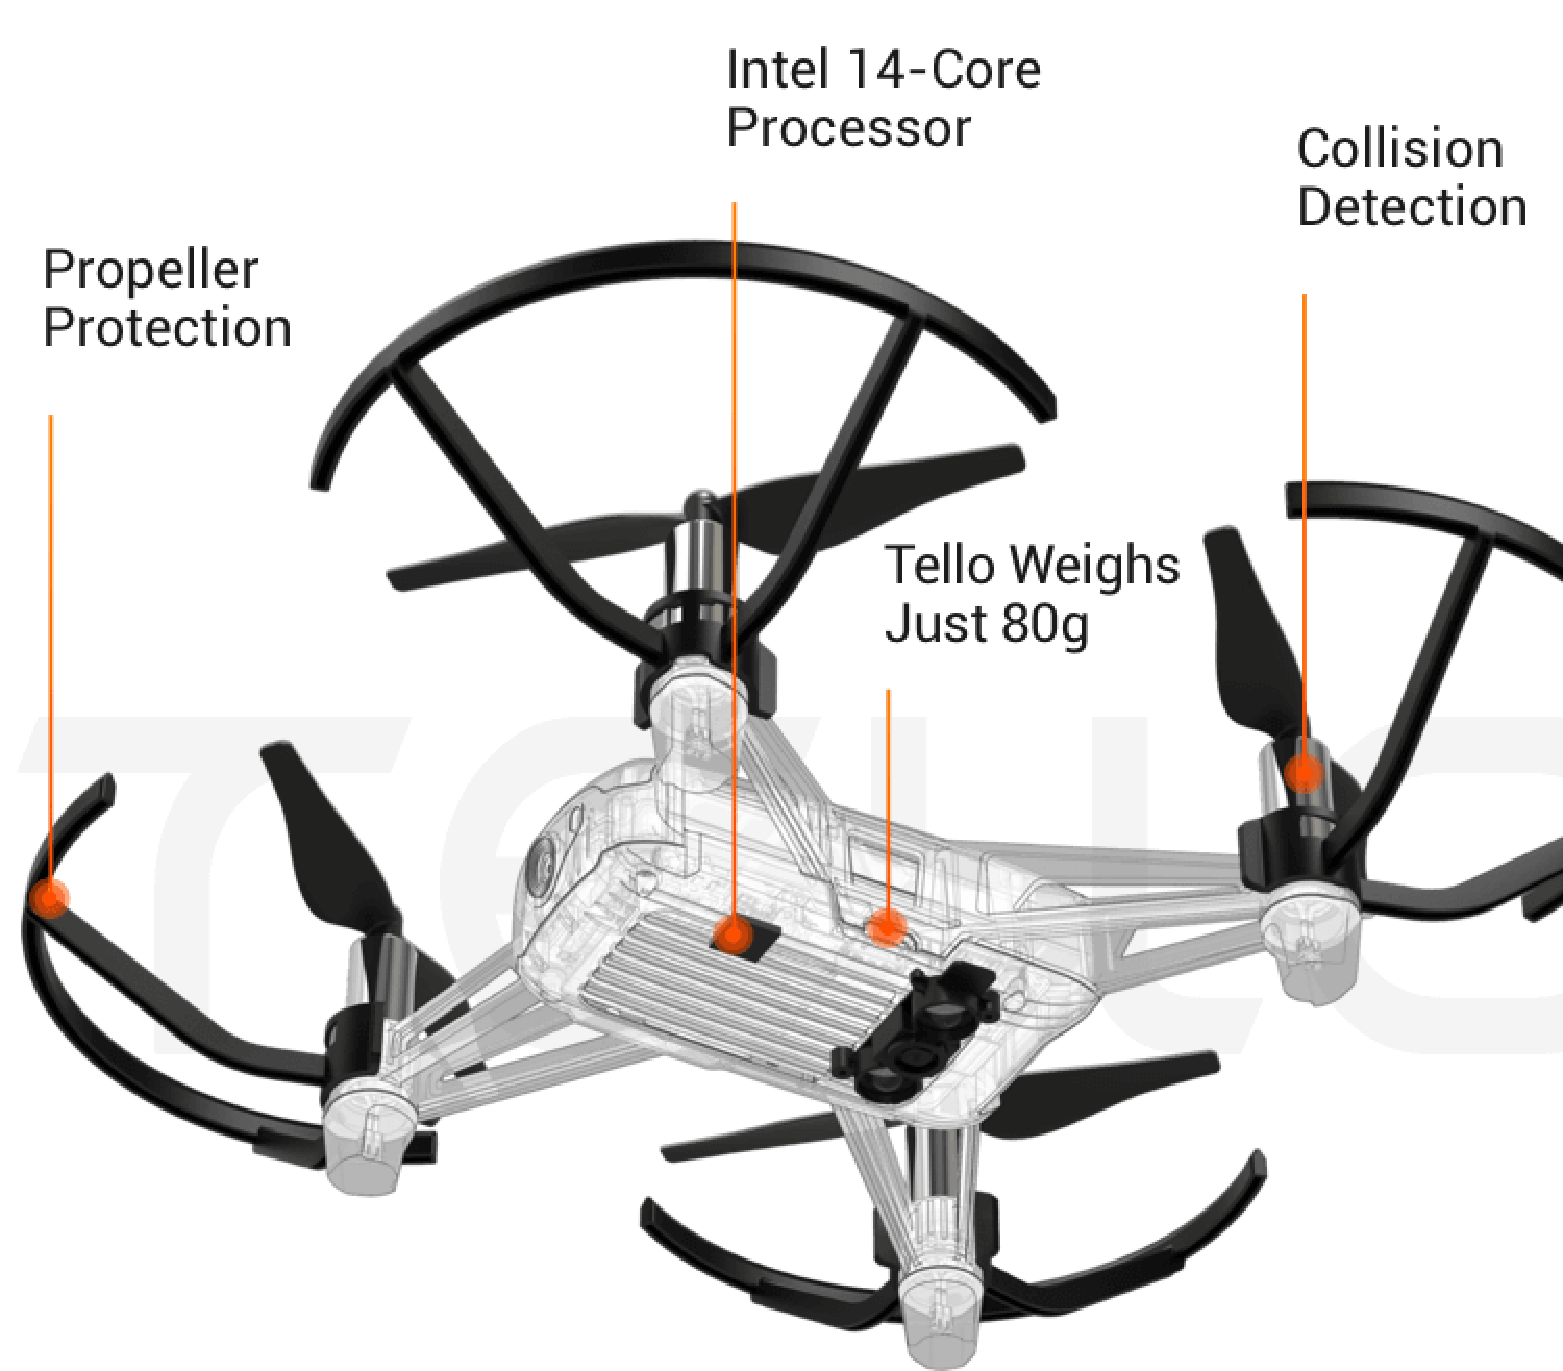
\includegraphics[width=.65\textwidth,angle=0]{figure 3-1.pdf}
\caption{Architektúra systému riadenia robotov.}
\label{o:31}
\end{figure}

\subsubsection{Popis samotných blokov}

\textbf{Príkazový blok.}
Príkazový blok je súčasťou ovládacieho rozhrania, ktoré umožňuje používateľovi komunikovať so zariadením pomocou tlačidiel a odosielať nimi požadovaný príkaz. Tento ovládač sa skladá z piatich tlačidiel pre päť príkazov: hore, dole, doľava, doprava a stop. Tlačidlá hore a dole sa používajú na príkaz robota, aby sa pohyboval dopredu a dozadu. Ľavé tlačidlo slúži na ovládanie robota pri odbočovaní doľava a pravé tlačidlo pri odbočovaní doprava. Na zastavenie robota je možné použiť tlačidlo Stop.
\vspace{1mm}

\justifying
\noindent
\textbf{Blok radiča.}
Blok radiča je prepojený s rozhraním, dekóduje príkazy a vydáva riadiace signály do príslušných modulov, aby sa robot
mohol pohybovať. Udržuje tiež časovanie a postupnosť generovania riadiacich signálov. Prijíma rozhodnutia na základe
príkazov na riadenie pohybu robota v ľubovoľnom smere.
\vspace{1mm}

\justifying
\noindent
\textbf{Blok mobility.}
Blok mobility sa skladá z motorov a kolies. Tento blok prijíma príkazy z ovládača a pomocou rovníc diferenčného pohonu
ich transformuje na hodnoty pre každý z motorov a priraďuje tieto hodnoty, ktoré umožňujú pohyb robota


\subsection{Režimy navigácie}
Úloha prenasledovania koristi je rozdelená na časti. Každý robot sa pohybuje v troch navigačných režimoch nasledovne
\begin{enumerate}
\item Režim detekcie koristi.
\item Režim prenasledovania a navigácie: Počas tohto režimu je robot riadený na sledovanie koristi.
\item Režim znehybnenia(chytenia) koristi: Toto je konečný režim, v ktorom roboty vytvárajú figúrku, ktorá korisť uzavrie.
\end{enumerate}

\begin{figure}[ht!]
\centering
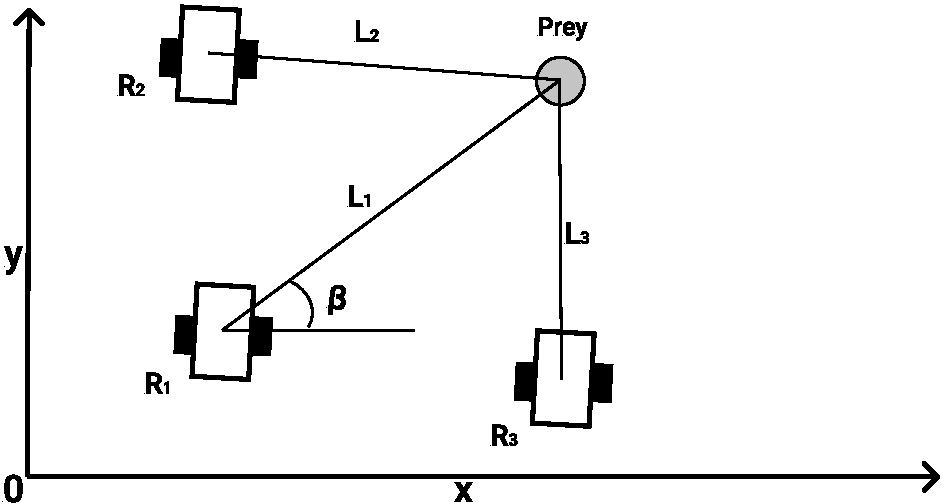
\includegraphics[width=.65\textwidth,angle=0]{figure 3-2.pdf}
\caption{Ilustrácia geometrie problému sledovania a navigácie.}
\label{o:32}
\end{figure}

Tieto režimy sú v ďalších častiach opísané osobitne.

\subsubsection{Režim detekcie koristi}

Pretože mobilný robot by mal vykonávať činnosť, je potrebné, aby robot vedel, aká je jeho poloha. Preto musí
mať implementovaný nejaký spôsob lokalizácie. Tieto metódy závisia od typu robota, od typu senzorov robota, od typu
súradnicového systému alebo od typu prostredia, v ktorom robot pracuje. V oblasti lokalizácie mobilných robotov sa
osvedčujú trigonometrické metódy, inerciálne navigačné metódy alebo matematicky komplikovaná
pravdepodobnostná metóda.

\vspace{3mm}

\justifying
\noindent
V súčasnosti má takmer každý novo vyvinutý mobilný robot zabudovaný kamerový systém. Preto je vhodné
ho použiť na
určenie polohy robota v prostredí. Vizuálna lokalizácia patrí do skupiny trigonometrických metód. Vizuálny systém môže
obsahovať jednu alebo dve kamery a mal by zisťovať niektoré značky v prostredí pomocou nástrojov počítačového videnia. Tieto značky môžu byť umelé alebo prirodzené (vrátane charakteristických vlastností prostredia, ktoré je
možné získať pomocou rôznych algoritmov). Ak vizuálny systém pozostáva iba z jednej kamery, rovnako ako v našom prípade,
poloha robota vo vzťahu k
značke sa počíta z dvoch snímok prostredia, v ktorom je počas pohybu robota jedna značka na rôznych miestach obrazu.

\vspace{3mm}

\justifying
\noindent
Ďalej je potrebné zabezpečiť, aby vzor kódujúci jedinečný identifikátor značky nemohol byť vytvorený rotáciou iného
vzoru používaného v prostredí. Tieto požiadavky sú splnené v systéme značiek zvaných ArUco, ktorý je založený na
AR-Tag a je dodávaný s knižnicou funkcií na detekciu a lokalizáciu značiek, ktorú sme používali na zisťovanie a
identifikáciu robotickej koristi v prostredí.

\vspace{3mm}

\justifying
\noindent
Simulačný algoritmus pozostáva z nasledujúcich postupných krokov (obrázok 3-3):
\begin{enumerate}
\item Priradenie interných a externých parametrov kamery (veľkosť snímača v pixeloch a milimetroch, ohnisková
vzdialenosť objektívu, koeficienty skreslenia, umiestnenie kamery).
\item Priradenie dvojrozmerných súradníc rohov známky v súlade s jej pôvodným obrázkom.
\item Priradenie trojrozmerných súradníc rohov známky v súlade s jej špecifikovanými fyzickými rozmermi.
\item Priradenie vymodelovanej 3D polohy značky pomocou vektora posunutia a rotácie.
\item Výpočet nových trojrozmerných súradníc rohov značky vynásobením počiatočných súradníc rotačnej a translačnej matice.
\item Projekcia trojrozmerných bodov rohov značky do dvojrozmerných bodov na modelovanom obrázku pomocou parametrov
kamery.
\item Výpočet funkcie transformácie perspektívy z dvojrozmerných súradníc pôvodu na projektované rohové súradnice.
\item Vykreslenie obrazu známky v nových dvojrozmerných súradniciach na upravenom obrázku pomocou perspektívnej
transformácie.
\item Odhad polohy 3D značiek pomocou detektora značiek na modelovanom obrázku.
\item Vyhodnotenie chyby porovnaním odhadovanej polohy značky s vopred určenou polohou v kroku 4.
\item Opakovanie krokov 4 až 10 pre ďalšie polohy značiek.
\end{enumerate}

\begin{figure}[ht!]
\centering
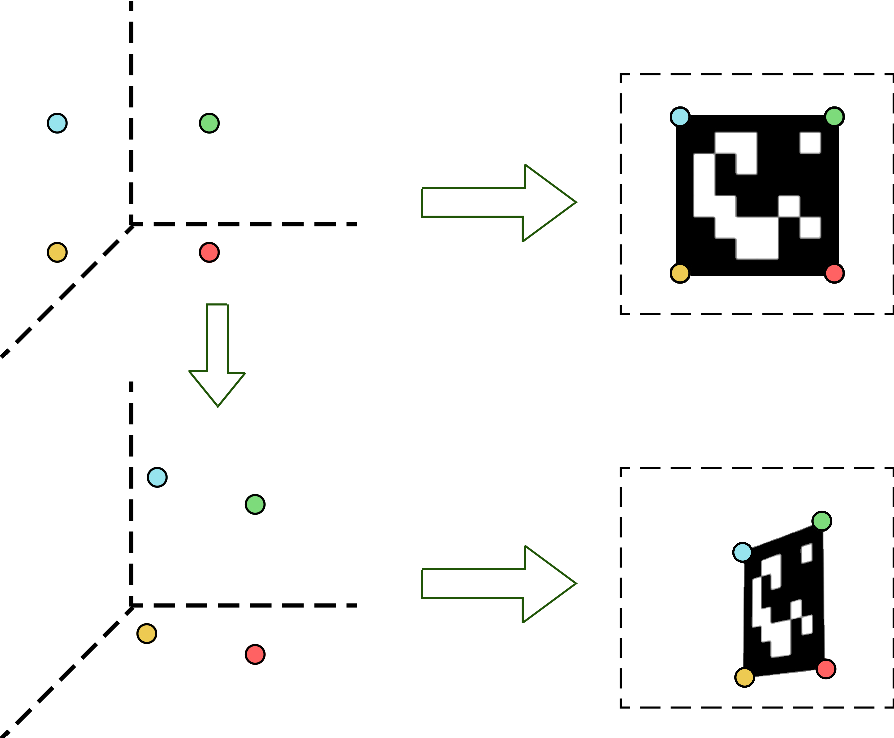
\includegraphics[width=.65\textwidth,angle=0]{figure 3-3.pdf}
\caption{Schéma modelovania obrázkov so značkami ArUco.}
\label{o:33}
\end{figure}

\vspace{3mm}

\justifying 
\noindent 
Interný binárny kód značky je definovaný piatimi slovami, každé z nich obsahuje päť bitov. Na zakódovanie identifikátora
sa používa mierna úprava Hammingovho kódu. Preto sú z piatich bitov slova iba dva nosiče užitočných informácií. Počet
jedinečných značiek sa teda rovná 1024 \citep{garido}.
Po úspešnej detekcii značky knižnice ArUco poskytujú informácie o polohe vzhľadom na optický stred kamery. Pre
rotáciu poskytuje systém ArUco štandardnú transformačnú maticu alebo štvorec. Na účely lokalizácie musia byť tieto údaje
transformované do Eulerových uhlov. Z hľadiska umiestnenia mobilných robotov je potrebné určiť rotáciu okolo osi z:
\begin{equation}\label{r:11}
\theta = \arctan{[2.(X.Y - W.Z), W^2-X^2-Y^2+Z^2]}
\end{equation}

\justifying
\noindent
Kde $W$, $X$, $Y$ a $Z$ sú prvky popisujúce štvorček poskytovaný funkciami knižnice ArUco. Poloha robota voči značke je
daná:
\begin{gather}\label{r:12}
x_w = x.cos(\theta) - z.sin(\theta); \\
y_w = z.cos(\theta) - x.sin(\theta); \\
\theta_w = \theta
\end{gather}
Kde $x$ je poloha značky vzhľadom na optické stretnutie fotoaparátu pozdĺž osi x, $z$ je vzdialenosť medzi fotoaparátom a rovinou kolmou na optickú os fotoaparátu a je pretínajúc stredom značky a $\theta$ je uhol medzi fotoaparátom a značkou (obrázok 3-4).
\begin{figure}[ht!]
\centering
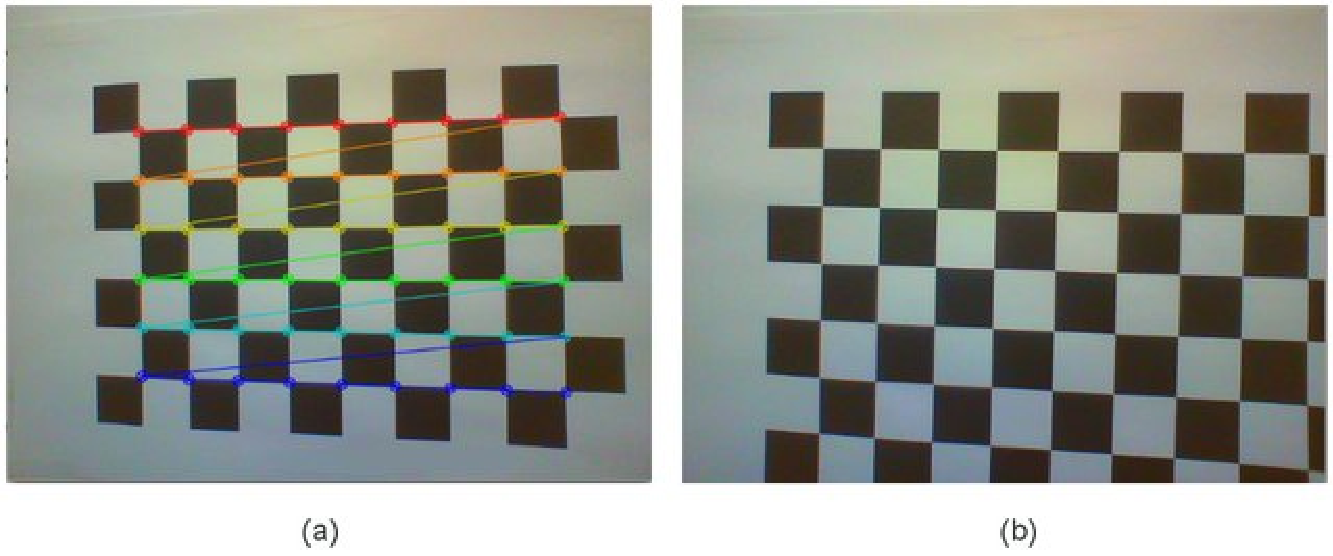
\includegraphics[width=.65\textwidth,angle=0]{figure 3-4.pdf}
\caption{Určenie polohy robota vzhľadom na značku.}
\label{o:34}
\end{figure}

\justifying
\noindent
Globálna poloha robota $x_w$, $y_w$ a $\theta_w$ podľa obrázku 3-5 je potom:
\begin{gather}\label{r:2}
x_w = x.cos(\theta_R + \theta_Z) - z.sin(\theta_R+\theta_Z) + x_Z; \\
y_w = z.cos(\theta_R + \theta_Z) - x.sin(\theta_R+\theta_Z) + y_Z; \\
\theta_w = \theta_R + \theta_Z
\end{gather}
\begin{figure}[ht!]
\centering
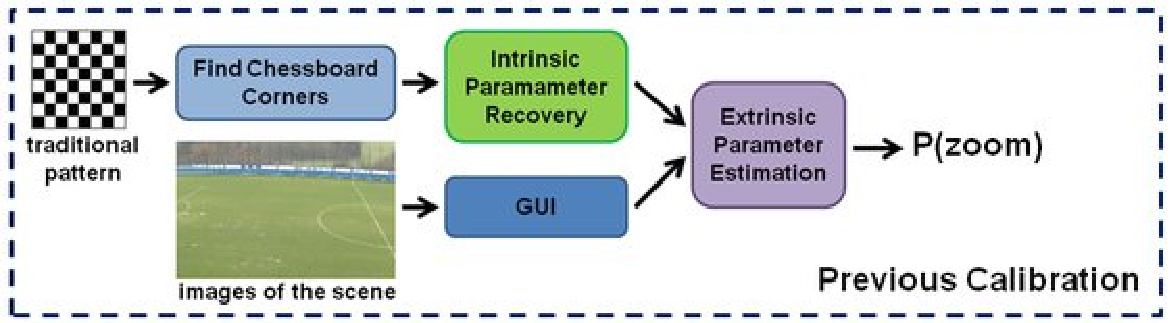
\includegraphics[width=.65\textwidth,angle=0]{figure 3-5.pdf}
\caption{Určenie globálnej polohy robota pomocou polohy značky.}
\label{o:35}
\end{figure}
\vspace{3mm}

\justifying
\noindent 
Pomocou údajov získaných výpočtom polohy robota vo vzťahu ku koristi - vykonajú roboty detekciu a sledovanie koristi.
\begin{figure}[ht!]
    \centering
    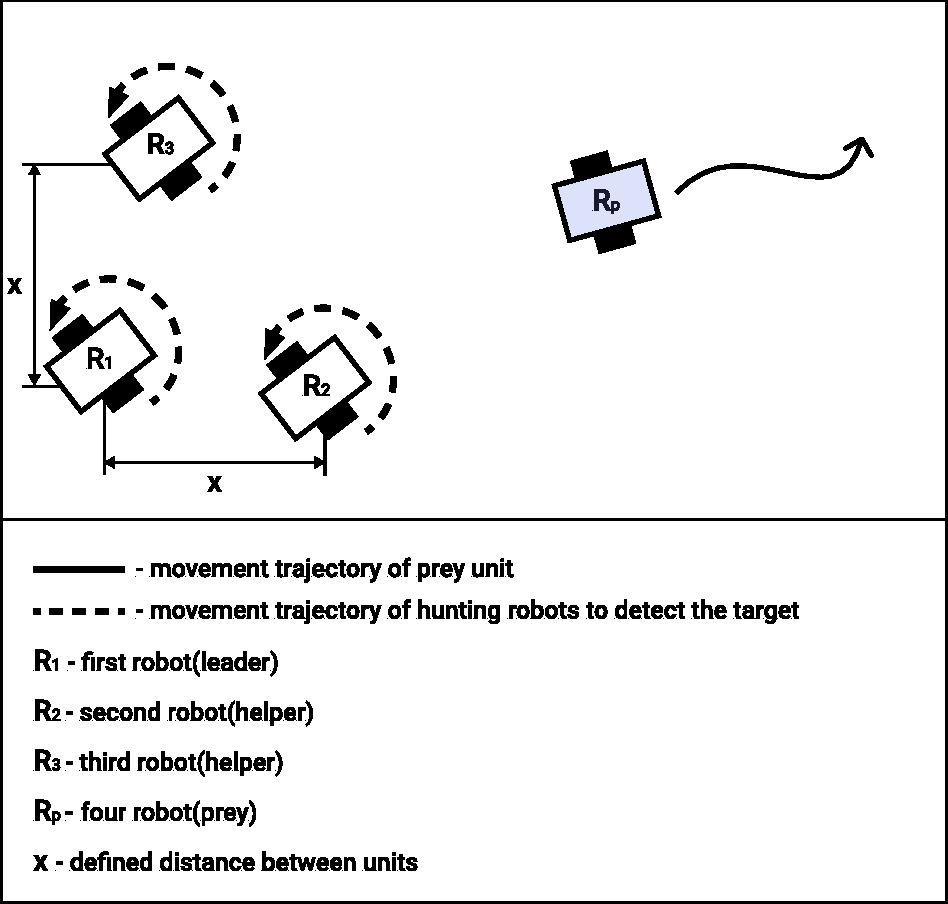
\includegraphics[width=.65\textwidth,angle=0]{scheme-1.pdf}
    \caption{Režim detekcie koristi - schéma.}
    \label{o:37}
\end{figure}

\subsubsection{Režim prenasledovania a navigácie}


Tento režim je pravdepodobne najdôležitejším režimom v rámci problému s lovom. Roboti začnú korisť sledovať zo svojich
počiatočných pozícií. Výpočet relatívnej
vzdialenosti od cieli a uhla vychýlenia sa vykonáva pomocou systému značiek AruCo, ktorý je podrobne popísaný v
predchádzajúcej časti.

\vspace{3mm}

\justifying
\noindent
Pretože sa prenasledovateľ bude pohybovať v smere uvedenom v oddiele 3.3.1, je potrebné, aby prenasledovateľ upravil
svoju rýchlosť iba v závislosti od svojej relatívnej polohy k cieľu. Aby sme zaručili, že prenasledovateľ nenarazí na
korisť, zavedieme bezpečnú vzdialenosť r (0 <r <R), takže keď je vzdialenosť medzi prenasledovateľom a korisťou menšia
ako r, prenasledovateľ by mal spomaliť o $\delta$, aby sa zväčšil ich vzdialenosť rýchlo. Rýchlosť sa potom nastavuje
odlišne podľa nasledujúcich troch podmienok: 
\begin{itemize}
    \item d(P, A) > R. V tejto situácii je vzdialenosť od prenasledovateľa po
    korisť veľmi veľká, čo sa často stáva v počiatočnej fáze sledovania, prenasledovateľ musí prenasledovať korisť
    zrýchlením. Rýchlosť prenasledovateľa sa v každom kroku prudko zvýši o to, aby sa dosiahlo rýchle zmenšenie
    vzdialenosti. Z dôvodu obmedzenia maximálnej zmeny rýchlosti by mala byť maximálna rýchlosť prenasledovateľa
    obmedzená, aby sa zabránilo kolízii do cieľa.
    \item r <= d (P, A) <= R. Toto je požadovaný stav prenasledovateľa. Pretože prenasledovateľ je už v bezpečnom dosahu ku
    koristi, musí iba nasledovať korisť porovnaním jej rýchlosti s rýchlosťou koristi.
    \item d (P, A) < r. V takom prípade sa prenasledovateľ drží príliš blízko ku koristi. Prenasledovateľ preto zníži svoju
    rýchlosť o maximum $\delta$ m/s, aby získal väčšiu manévrovateľnosť z hľadiska bezpečnosti. Algoritmus 1 sumarizuje
    navrhovanú schému sledovania koristi-predátora.
\end{itemize} 

\vspace{3mm}

\justifying
\noindent
V prírode môže lovcovi občas chýbať snímanie koristi v dôsledku oklúzie. Pri robotickom sledovaní môže komunikácia medzi robotmi z času na čas zlyhať. V týchto situáciách s neistotou vnímania musí prenasledovateľ predvídať trajektóriu cieľa, aby mohol pokračovať v úlohe sledovania. Predpovedaním trajektórie cieľa môže prenasledovateľ približne sledovať cieľ pri neistote vnímania, a preto zvyšuje odolnosť a kontinuitu sledovania. Keď sa vnímanie vráti do normálneho stavu, prenasledovateľ rýchlo napraví chyby sledovania bez vykonania fázy naháňania, ktorá zvyčajne trvá dlhšie.
V tomto projekte začleňujem do našej sledovacej schémy prediktívne schopnosti. Keď je korisť vnímaná, prediktívny model sa učí predpovedať jej aktuálnu polohu na základe jej predchádzajúceho správania. Akonáhle korisť nie je vnímateľná, naučený model sa použije na predpovedanie neznámej polohy.
Existujú tri metódy:
\begin{enumerate}
    \item Jednoduchá inferencia.
    \item Autoregresívny model.
    \item Echo stavové siete. 
\end{enumerate} 
V tomto projekte používa sa jednoduchá inferencia. Keď sú informácie o koristi na krátky čas nedostupné, existuje veľmi jednoduchá hypotéza, že zachová rovnaký trend lineárneho pohybu s konštantnou rýchlosťou. Inými slovami, posledná pozorovaná rýchlosť a smer budú fungovať ako odhad neznámej rýchlosti a smeru počas tohto časového obdobia.
Tento predpoklad je veľmi jednoduchý a intuitívny. Pochádza z prirodzeného sledovania človekom. Ľudia budú pokračovať v sledovaní za predpokladu, že cieľ bude pokračovať v ceste rovnakým smerom a rovnakou rýchlosťou, keď nebudú môcť cieľ vidieť. Tento predpoklad je ale užitočný iba v situáciách, keď pozorovanie chýba veľmi krátko. Ďalšou výhodou tejto metódy je, že nie je potrebné žiadne učenie, takže je výpočtovo efektívnejšia ako ostatné dve predikčné metódy. 

\begin{figure}[ht!]
    \centering
    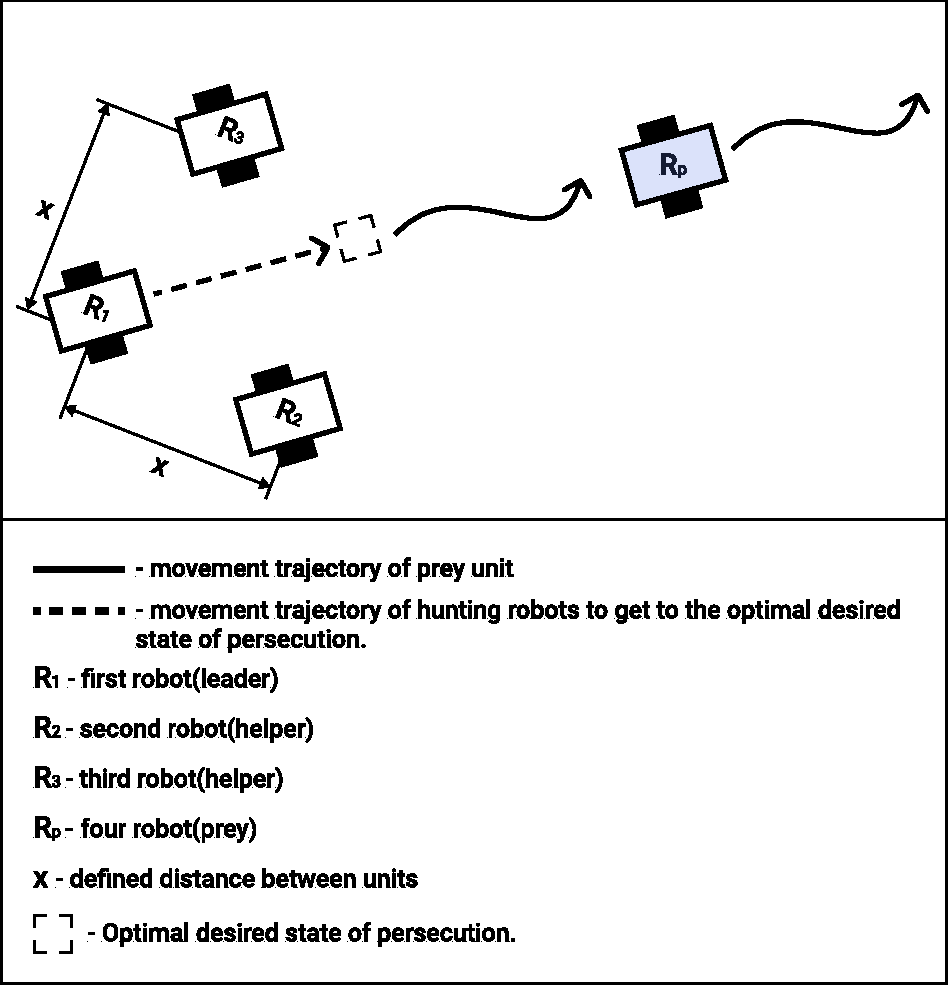
\includegraphics[width=.75\textwidth,angle=0]{scheme-2.pdf}
    \caption{Režim sledovania a navigácii - schéma.}
    \label{o:38}
\end{figure}

\subsubsection{Režim znehybnenia (chytenia) koristi}

Toto je posledný režim navigácie, kde je cieľom robotov uzavrieť korisť. Problém je tu zložitejší, pretože cieľom je sformovať postavu okolo pohybujúceho sa objektu. Tento režim sa aktivuje pre každého robota osobitne, keď robot dosiahne bod v rámci danej vzdialenosti od koristi (povedzme 10). Kruh obklopujúci korisť má ako polomer 10. Tvorba kruhu sa ustanovuje v nasledujúcich krokoch:
\begin{enumerate}
    \item Vzhľadom na počet robotov a vzdialenosť $l_0$ sa počíta
        neskoro $l_1$, vzdialenosť medzi dvoma po sebe nasledujúcimi robotmi vo formácii.
    \item Keď roboti dosiahnu bod so vzdialenosťou $l_0$ od
        korisť, aktivuje sa režim formovania kruhu. Roboty vykonávajú zložitý pohyb, aby udržali vzdialenosť od koristi konštantnú a rovnú $l_0$ a súčasne sa vytvorili
        jednotný kruh okolo koristi.
    \item Po dosiahnutí formácie - vykonajú roboti rovnaký typ pohybu ako korisť obklopená robotmi. 
\end{enumerate} 

\begin{figure}[ht!]
    \centering
    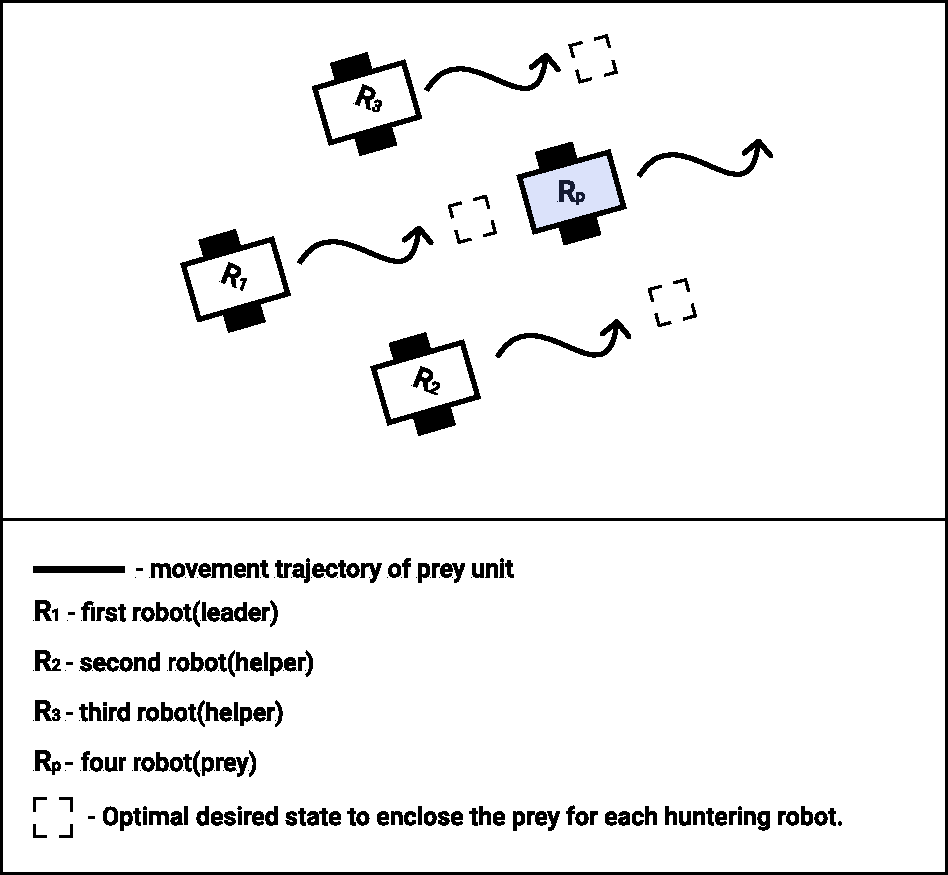
\includegraphics[width=.75\textwidth,angle=0]{scheme-3.pdf}
    \caption{Režim zatváranie koristi - schéma.}
    \label{o:39}
\end{figure}

\subsection{Výber vhodnej metódy robotickej kooperácie}
V tejto časti sa budeme zaoberať metódami použitými pri prace nad projektom, analyzujeme tiež výhody a nevýhody rôznych metód a urobíme odôvodnenú voľbu v prospech určitých riešení s prihliadnutím na špecifikáciu vypracovaného projektu.

\subsubsection{Centralizované vs. decentralizované}
Pre návrh na vysokej úrovni, používa sa zmiešaný riadiaci systém. To riadenie na vysokej úrovni spočíva v ovládaní globálnych parametrov a koordinácii robotov pomocou 
základňovej stanice, ako je spracovanie prijatých snímok z kamery, koordinácia a aktivácia režimov pohybu robota, 
koordinácia pohybov skupiny robotov. Zároveň sú roboty schopné navzájom si prenášať miestne parametre a údaje senzorov.
Tento režim bol vybraný, pretože s úplným centralizovaným riadením môžu nastať problémy s rýchlosťou príjmu údajov od všetkých robotov súčasne. 
A nepoužíva sa decentralizovaný systém, pretože je ťažké v ňom koordinovať prácu všetkých robotov a spracovanie informácií prebieha na samotnom robotovi, 
čo zvyšuje požiadavky na výpočtovú schopnosť takého robota. Ako výsledok návrh na vysokej úrovni bude využívať systém spätnej väzby. 
\begin{figure}[ht!]
    \centering
    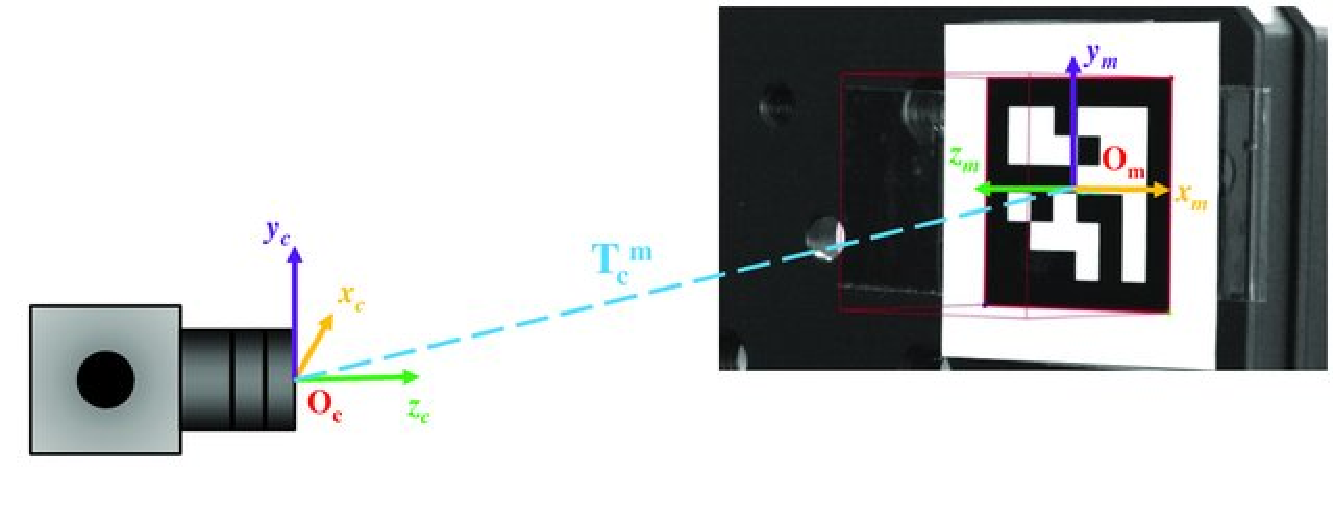
\includegraphics[width=.75\textwidth,angle=0]{figure 3-6.pdf}
    \caption{Hybridná architektúra riadenia.}
    \label{o:310}
\end{figure}

\subsubsection{Systém spätnej väzby(Closed-Loop Control System)}
Dizajn s uzavretou slučkou využíva systém spätnej väzby. Spätná väzba umožňuje systému určiť súčasné a budúce reakcie systému na základe súčasných alebo minulých informácií. Je to prospešné, pretože sa zvyšuje presnosť a spoľahlivosť výstupu, pretože systém sa môže sám prispôsobiť tak, aby získal požadovaný výkon. Systém s otvorenou slučkou môže robiť úpravy iba na základe vopred naprogramovaných nastavení a nemôže zohľadňovať zmeny prostredia alebo situácie.
Rozhodol som sa implementovať riadiaci systém uzavretej slučky pre robotov. Poloha koristi a robotov sa bude meniť od behu k behu, preto je potrebné mať spätnú väzbu. Okrem toho je dôležité zhromažďovať údaje o spätnej väzbe o rýchlosti robota, aby bolo možné vykonať úpravy, aby sa roboty pohybovali správne. 
\begin{figure}[ht!]
    \centering
    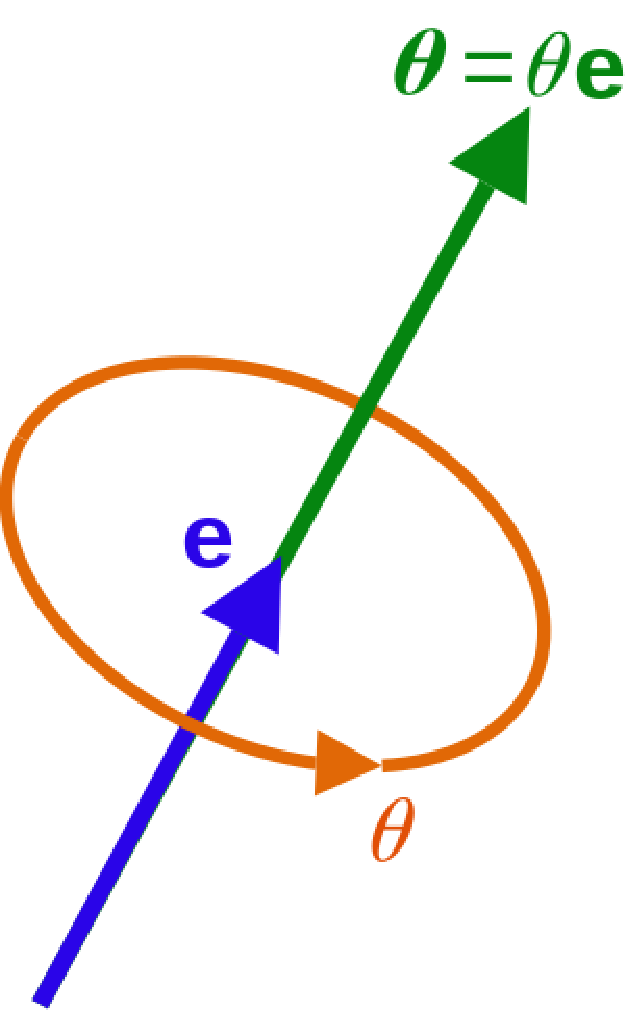
\includegraphics[width=.75\textwidth,angle=0]{figure 3-7.pdf}
    \caption{Systém spätnej väzby.}
    \label{o:311}
\end{figure}

\subsubsection{Deliberatívne vs. reaktívne riadenie}
V tomto prípade sa používa reaktívny riadiaci prístup, pretože zámerný riadiaci prístup založený na plánovaní pohybu a trajektórie pohybu si vyžaduje predbežné 
znalosti prostredia, aby bolo možné plánovať pohyby robotov, čo pre  tento projekt nie je 
možné. Pomocou reaktívneho riadenia som sa rozhodol implementovať hierarchickú pohybovú 
stratégiu, v ktorej, ako sme diskutovali v časti 2.4.2, je jeden robot považovaný za vedúceho a 
ostatní roboti sú druhí. Vodca zvyčajne sleduje trajektóriu a nasledovníci sledujú jeho 
transformované súradnice. 